\documentclass[main.tex]{subfiles}
\begin{document}

\section{The equation of state and degenerate gasses}

\marginpar{Tuesday\\ 2020-10-20, \\ compiled \\ \today}

% Still no answer about the quadrupole stuff

% 151879

We move away from the relativistic realm, and treat the more classical Equation of State (EoS). 
In general \(P\) could be a function of \(\rho \), \(\mu \), \(T\) and other variables. 
An often-used one is \(P = P (\rho )\); also sometimes we use \(u = u(\rho )\), where \(u\) is the internal energy density. 

We will treat the equation of state of a completely degenerate gas. 

Let us start for a very simple system: a \textbf{hydrogen plasma}. 
It is a collection of \(e^{-}\) and protons \(p\). 

We have complete collisional ionization for \(T \gtrsim \SI{e5}{K}\). 
Under which conditions is this plasma relativistic or nonrelativistic? This is shown as the blue area in figure \ref{fig:relativisticity_degeneracy}.

The electrons are surely relativistic if \(k_B T \gtrsim m_e c^2\), which corresponds to \(T \gtrsim \SI{6e9}{K}\). 
For the protons, an analogous equation yields \(T \gtrsim \SI{e13}{K}\): these temperatures are basically never reached for realistic astrophysical scenarios. 

\begin{figure}[ht]
\centering
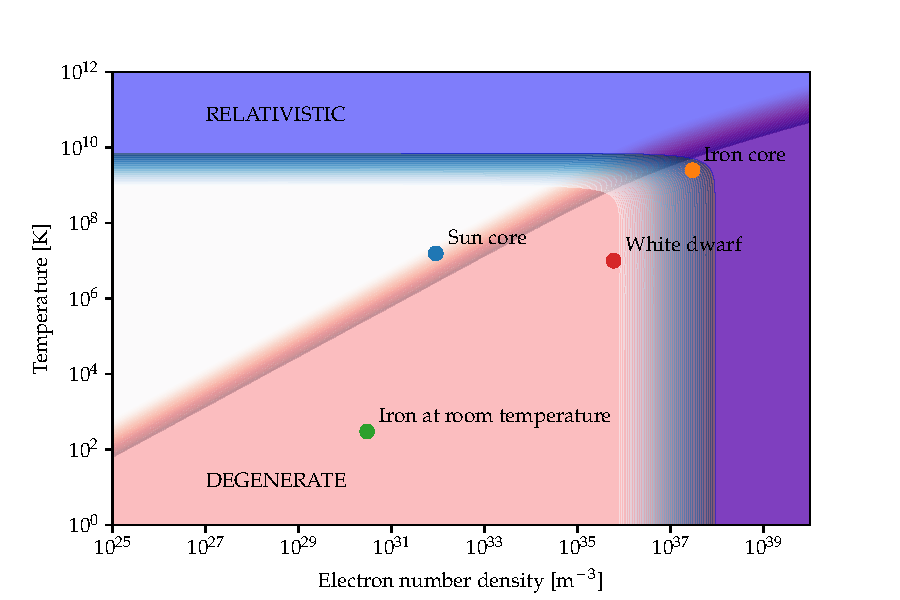
\includegraphics[width=\textwidth]{figures/relativisticity_degeneracy.pdf}
\caption{}
\label{fig:relativisticity_degeneracy}
\end{figure}

In the region of \(\SI{e5}{K} \lesssim T \lesssim \SI{e9}{K}\) (for low densities), the plasma will be ionized but not relativistic. 

The ideal gas law for the electrons reads \(P_e = n_e k_B T\), for the ions \(P_i = n_i k_B T\). 
However, electrons are much lighter than protons, so for the same forces they will accelerate more, so they will radiate away more energy. 

Another complication is the following: consider a collection of \(N\) ionic species, then for each of these (labelled by \(k\)) we will have \(P_{i, k}= n_{i, k} k_B T\). 
The total pressure can be calculated by summing over all of these, plus the electrons: 
%
\begin{align}
P &= n_e k_B T + \sum _{k} n_{i, k} k_B T = k_B T \qty(n_e + \sum_k n_{i, k})  \\
&= \frac{nk_B T}{\mu }
\,,
\end{align}
%
where \(\mu \) is the \emph{mean molecular weight}, calculated through the total baryonic number density \(n\): 
%
\begin{align}
\mu = \qty[\frac{n_e}{n} + \frac{\sum _{k} n_{i, k}}{n} ]^{-1}
\,.
\end{align}

For a pure hydrogen plasma, we have one electron per proton, so we find 
%
\begin{align}
\mu_{\ce{H}} = \qty[1 + 1]^{-1} = \frac{1}{2}
\,.
\end{align}

For a pure helium plasma we have two electrons per Helium nucleus, which contains 4 baryons: so, 
%
\begin{align}
\mu_{\ce{^{4}He}} = \qty[ \frac{2}{4} + \frac{4}{4}]^{-1} = \frac{4}{3}
\,.
\end{align}

This holds under the assumption that the plasma behaves like an ideal gas, and that the electrons and protons are nonrelativistic. 
There is a crucial reason why the first assumption fails: \textbf{degeneracy}.

Electrons obey Dirac statistics, and if the density is high enough they can behave very similarly to the \(T = 0\) limit even for high temperatures. The region in which they behave like a fully degenerate gas is shown in pink in figure \ref{fig:relativisticity_degeneracy}. 

The distribution function for a system of fermions reads 
%
\begin{align}
\frac{ \dd{N}}{ \dd[3]{x} \dd[3]{p}} = \frac{2}{h^3} \underbrace{\qty[\exp(\frac{E }{k_B T} - \alpha ) + 1]^{-1}}_{f}
\,.
\end{align}

Here, the \emph{degneracy parameter} is \(\alpha = \mu / k_B T\), where \(\mu  \) is the chemical potential. 
The energy is expressed as \(E = \sqrt{m^2 c^{4} + p^2 c^2}\).

If we want to compute \(\alpha \), we can just integrate: 
%
\begin{align}
n &= \int_{\mathbb{R}^3} \frac{ \dd{N}}{ \dd[3]{x} \dd[3]{p}} \dd[3]{p}  \\
&= \frac{2}{h^3} \int_0^{\infty } 
\qty[\exp(\frac{E }{k_B T} - \alpha ) + 1]^{-1} 4 \pi p^2 \dd{p}
\,.
\end{align}

This integral can be computed for any value of \(\alpha \) and \(T\): we then find \(n = n(\alpha , T)\). Inverting this relation, we find \(\alpha = \alpha (n, T)\). 

The logarithm of the absolute value of \(\alpha k_B T = \mu \) can be plotted against \(\log n\) for different values of the temperature \(T\). For each \(T\), there is a cusp: \(\alpha \) changes sign. It can become very big and positive or very big and negative. 

\todo[inline]{Do plot!}

Let us start with the case \(\abs{\alpha } \gg 1 \) and \(\alpha < 0\): this corresponds to low \(n\), high \(T\). 
Then, the \(- \alpha \) appearing in the distribution is large and positive: then, the distribution looks like \(f \sim \exp(- \frac{E}{k_B T})\), the Maxwell-Boltzmann distribution. 
The gas is behaving like an ideal gas. 

Another option is \(\abs{\alpha } \gg 1\), \(\alpha > 0\). This is the case in which we have low \(T\), high \(n\). Even in the \(T \to 0\) limit, the product \(\alpha k_B T \) stays finite: this is a function of \(n\), and is called \(E _F\).

The distribution then looks like \(f \sim \qty[\exp( (E - E_F) / k_B T) + 1]^{-1} \to [E \leq E_F]\) in the limit \(T \to 0\).
(I use the Iverson bracket: \([\text{proposition}]\) is 1 if the proposition is true, 0 if it is false).  

The higher \(n\) is, the higher the \(T\) for which the behavior is close to the \(T \to 0\) limit. 

In the \(T \to 0\) limit, we can do the integration analytically: this yields an explicit expression for \(n\) in terms of the Fermi momentum \(p_F\) corresponding to the Fermi energy \(E_F\): inverting it we get
%
\begin{align}
p_F = \sqrt[3]{\frac{3n }{8 \pi }} h
\,.
\end{align}

This momentum is a characteristic of \(n\) independently of the temperature: for \(T > 0\) it will not be a hard limit anymore, but it is still a good descriptor of the Fermi gas. 

We can write 
%
\begin{align}
E_F = \sqrt{m^2 c^{4} + p_F^2 c^2} = \sqrt{1 + x_F^2} m c^2
\,,
\end{align}
%
where \(x_F = p_F / mc^2\).
For a nonrelativistic particle distribution \(x_F \ll 1\), so \(E_F \approx mc^2 + x_F^2 mc^2/2\). 
The dependence on the number density of the kinetic part is \(\sim x_F^{2} \sim n^{2/3}\). 

On the other hand, in the ultrarelativistic limit \(E_F \approx x_F mc^2 \sim x_F \sim n^{1/3}\).

This is the reason why in figure \ref{fig:relativisticity_degeneracy} the pink boundary curves down in the blue (relativistic region). 

It is useful to define this quantity in terms of proper density, in \SI{}{g/cm^3}, instead of number density.

We have 
%
\begin{align}
x_F = \frac{p_F}{mc^2} = \qty( \frac{3h^3}{8 \pi })^{1/3} \frac{1}{mc^2} n^{1/3}
\,;
\end{align}
%
if we multiply above and below by the mean baryon mass, we have 
%
\begin{align}
n_e = \frac{n m_b}{m_e m_b} = \frac{\rho}{m_e m_b} 
\,,
\end{align}
%
which gives us 
%
\begin{align}
x_F \sim \num{e-2} \qty(\frac{\rho }{m_e})^{1/3}
\,.
\end{align}

\todo[inline]{Are we sure about this? I think I missed something.}

The internal energy density \(u\) is computed in general as 
%
\begin{align}
u &= \frac{2}{h^3}\int E(p) \frac{ \dd{N}}{ \dd[3]{x} \dd[3]{p}} \dd[3]{p} 
\,,
\end{align}
%
which in our case is 
%
\begin{align}
u &= \frac{2}{h^3} \int_{0}^{p_F} \sqrt{m^2c^{4} + p^2c^2} 4 \pi p^2 \dd{p}  \\
&= \frac{8}{h^3} \pi  mc^2 (mc)^3 \int_0^{p_F} \sqrt{1 + x^2} x^2 \dd{x}  \\
&= \frac{8 \pi m^4 c^{6}}{h^3} \frac{x_F^{4}}{4} I(x_F)
\,,
\end{align}
%
where \(I(x_F)\) can be computed analytically, but it is of order 1 as can be seen by the asymptotics of the integral. 

The integral reads 
%
\begin{align}
\int_0^{p_F} \sqrt{1 + x^2} x^2 \dd{x} = \frac{1}{8} \qty[x_F (1 + 2 x_F)^2 \sqrt{1 + x_F^2} - \log(x_F + \sqrt{1 + x_F^2})]
\,.
\end{align}

For the pressure we have a similar integral, which however is more complicated from the conceptual point of view. 

The first law of thermodynamics states that 
%
\begin{align}
\dd{U} + p \dd{V} = 0
\,,
\end{align}
%
as long as the transformation does not exchange heat with its surroundings. 
Note that \(\dd{u} = \dd{(U/ V)} = V^{-1} \dd{U} - U V^{-2} \dd{V}\), which means that 
%
\begin{align}
\frac{ \dd{U}}{V} = \dd{u} + \frac{U}{V} \dd{V}
\,.
\end{align}

Substituting into the first law of thermodynamics, 
%
\begin{align}
\dd{u} + \frac{U}{V} \dd{V} + P \dd{V} = 0
\,,
\end{align}
%
but since \(V \propto 1/n\) we have 
%
\begin{align}
\frac{ \dd{V}}{V} = - \frac{ \dd{n}}{n}
\,.
\end{align}

Substituting this in, we get 
%
\begin{align}
\dd{u} - (P+u) \frac{ \dd{n}}{n} = 0 
\,.
\end{align}

This means that 
%
\begin{align}
n \frac{\dd{u}}{ \dd{n}} = P + u
\,,
\end{align}
%
which allows us to compute the pressure! 
The only step remaining is to replace \(\dd{n} / n\) with an expression in terms of \(x_F\), which is 
%
\begin{align}
\frac{ \dd{x_F}}{x_F} = 3 \frac{ \dd{n}}{n}
\,.
\end{align}

This finally yields 
%
\begin{align}
P = \frac{x_F}{3} \dv{u}{x_F} - u
\,.
\end{align}

Then we are almost done: we can compute the pressure with \(u\), for which we have an analytic expression, and \(\dv*{u}{x_F}\), which we can easily find since the original expression for \(u\) was an integral in \(\dd{x_F}\), from which we can read off the integrand. 

This yields 
%
\begin{align}
P &= \frac{8 \pi m^4 c^{5}}{h^3} \qty[ 
    \frac{1}{3} x_F^3 \sqrt{1 + x_F^2 } 
    - \frac{1}{8} \qty(x_F (1 + 2 x_F)^2 \sqrt{1 + x_F^2} 
    - \log(x_F + \sqrt{1 + x_F^2}))
]  \\
&= \frac{m^4 c^{5} \pi }{h^3}
\qty[
    x_F \sqrt{1 + x_F^2}
    \qty( \frac{8}{3} x_F^2 - \qty(1 + 2 x_F^2))
    + \log(x_F + \sqrt{1 + x_F^2})
]  \\
&= \frac{m^4 c^{5} \pi }{h^3} \qty[
    x_F \sqrt{1+ x_F^2} 
    \qty( \frac{2}{3} x_F^2 - 1)
    +
    \log(x_F + \sqrt{1 + x_F^2})
]
\,.
\end{align}

\end{document}
